\documentclass{article}
\usepackage{graphicx}
\usepackage{marvosym}
\usepackage{dingbat}

\title{The MergeSort algorithm}
\date{}

\begin{document}

\maketitle
Mergesort is a divide and conquer algorithm for sorting the element of
an array. It can be implemented as a recursive procedure where the
input array is split in two halves, mergesort is recursively called
separately on each half and then the results of the two recursive calls
are combined together to build the final sorted array. 

\vspace{0.5cm}

\begin{minipage}{1.0\linewidth}
  \centering
  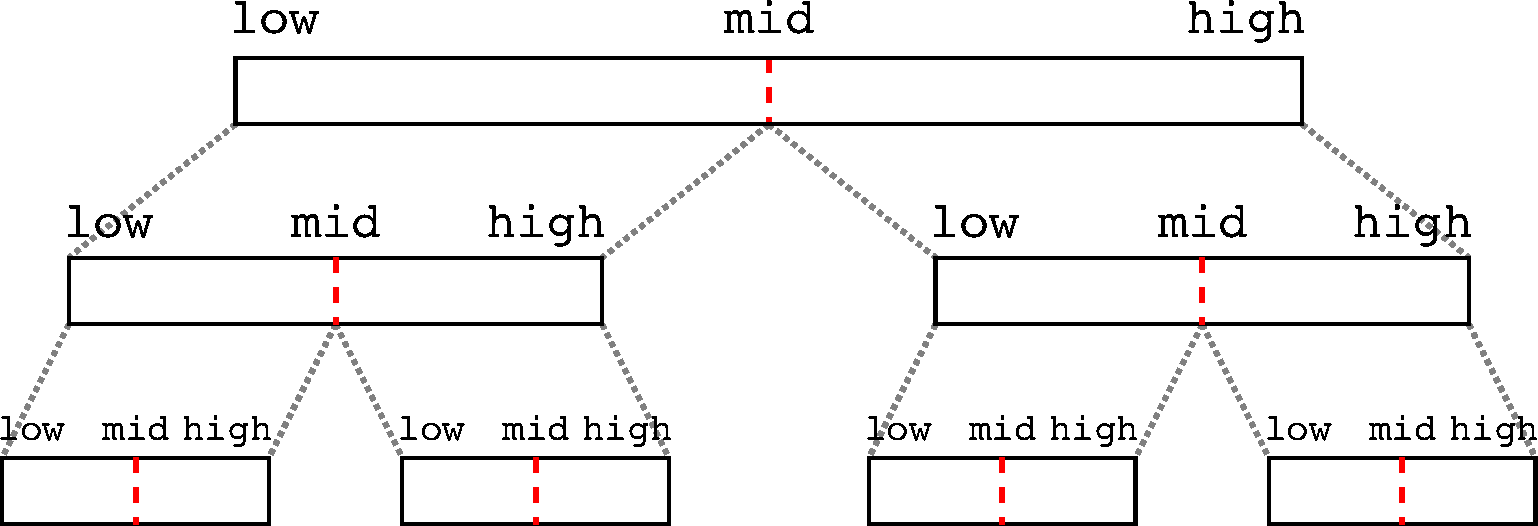
\includegraphics[width=0.8\textwidth]{msort}
\end{minipage}

The objective of this exercise is to parallelize the mergesort
algorithm using OpenMP.

\section{Package content}
The \texttt{MergeSort} directory contains a single file named
\texttt{mergesort.c}. This file contains a main program that allocates
an array, fills it with random numbers and then sorts it using the
mergesort algorithm. The mergesort algorithm is implemented through
the two routines \texttt{mergesort} and \texttt{merge}; only the first
one has to be modified to parallelize the algorithm.

The code can be compiled using the \texttt{make} command: simply type
\texttt{make} inside the \texttt{MergeSort} directory. This will
generate an executable \texttt{main} file that can be launched like
this
\begin{verbatim}
$ ./main n
\end{verbatim}
where \texttt{n} is the size of the array to be sorted. When executed,
the program will print the mergesort execution time or an error
message in case the result is not correct.

\section{Assignment}
\begin{itemize}
\item {\huge \Keyboard} parallelize the \texttt{mergesort} routine
  using the \texttt{\#pragma omp task} construct. Compile and run the
  \texttt{main} program using 1, 2 and 4 threads to verify that the
  proposed parallelization is correct. 
\item \smallpencil Evaluate the performance for a large value of
  \texttt{n} (up to 10M) of the parallelization
  using 1, 2 and 4 threads. Report the measured eecution times in the
  \texttt{responses.txt} file.
\end{itemize}


\section{Advice}
\begin{itemize}
\item Note that creating and handling tasks has a cost. It may be wise
  to limit the generation of tasks once a sufficient amount of
  parallelism has been reached.
\end{itemize}



\end{document}

%%% Local Variables: 
%%% mode: latex
%%% TeX-master: t
%%% End: 
